% !TEX program = xelatex

\documentclass[12pt, a4paper]{article}

\usepackage{fontspec}
\setmainfont[Ligatures=TeX]{Linux Libertine O}

\usepackage[colorlinks = true, urlcolor = blue]{hyperref}
\usepackage{indentfirst}
\usepackage{graphicx}
\usepackage[left=2cm,right=2cm,top=2.5cm,bottom=2.5cm]{geometry}
\usepackage{lipsum}

%\setlength{\parindent}{1em}
%\setlength{\parskip}{1em}\title{Εργασία Στατιστικής}

%\title{Java socket programming \\ 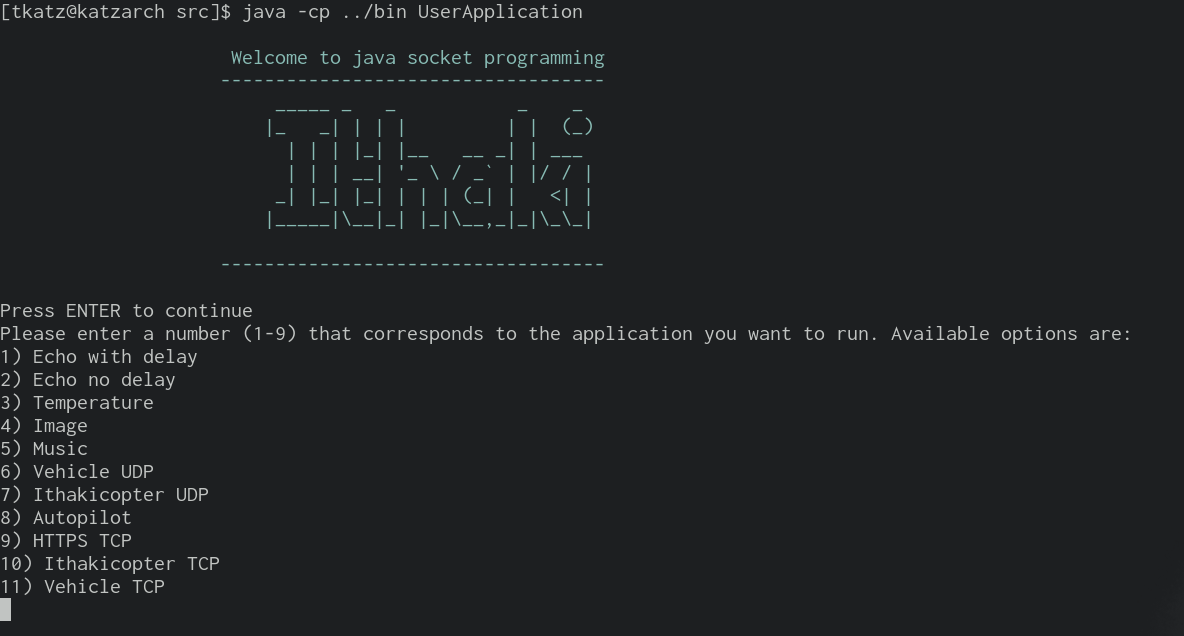
\includegraphics[width=\textwidth]{assets/login.png}}
% \author{Θεόδωρος Κατζάλης \\ ΑΕΜ:9282 \\ katzalis@auth.gr}
% \date{19/07/2020}

\begin{document}

\begin{titlepage}

\begin{figure}[h!]
  \begin{center}
    
\includegraphics[width=3cm]{assets/auth.pdf}
    \label{fig:cover_auth_logo}
  \end{center}
\end{figure}

\centering
\Large Αριστοτέλειο Πανεπιστήμιο Θεσσαλονίκης\\
\Large Πολυτεχνική Σχολή\\
%\large Τμήμα Ηλεκτρολόγων Μηχανικών και Μηχανικών Υπολογιστών\\
%\large Τομέας Τηλεπικοινωνιών

\vspace{\fill}

\LARGE \textbf{Java socket programming} \\
\LARGE \textbf{Δίκτυα 2}

\vspace{\fill}

\Large Θεόδωρος Κατζάλης \\
\Large ΑΕΜ:9282 \\ 
\Large katzalis@auth.gr

\vspace{\fill}
\raggedright

\centering
\vspace{\fill}
\today

\end{titlepage}

%\maketitle


\pagebreak
\tableofcontents{}
\pagebreak

\section{Lorem}
\lipsum


\section{Εισαγωγή}

Η συγκεκριμένη εργασία αποσκοπεί στην εξοικείωση εννοιών σχετικά με τα δίκτυα υπολογιστών τόσο σε θεωρητικό όσο και σε πρακτικό επίπεδο. Το πρώτο εξασφαλίζεται με την μελέτη και παράθεση βιβλιογραφίας σε πρωτόκολλα επικοινωνίας \textbf{TCP} και \textbf{UDP} ενώ το δεύτερο εξασφαλίζεται, χρησιμοποιώντας την γλώσσα προγραματισμού \textbf{java}, με την δημιουργία δικτυακών εφαρμογών συλλογής πληροφοριών απο τον server του μαθήματος ithaki με IP 155.207.18.208.

\section{User Interface}

\begin{figure}[h!]
\centering
	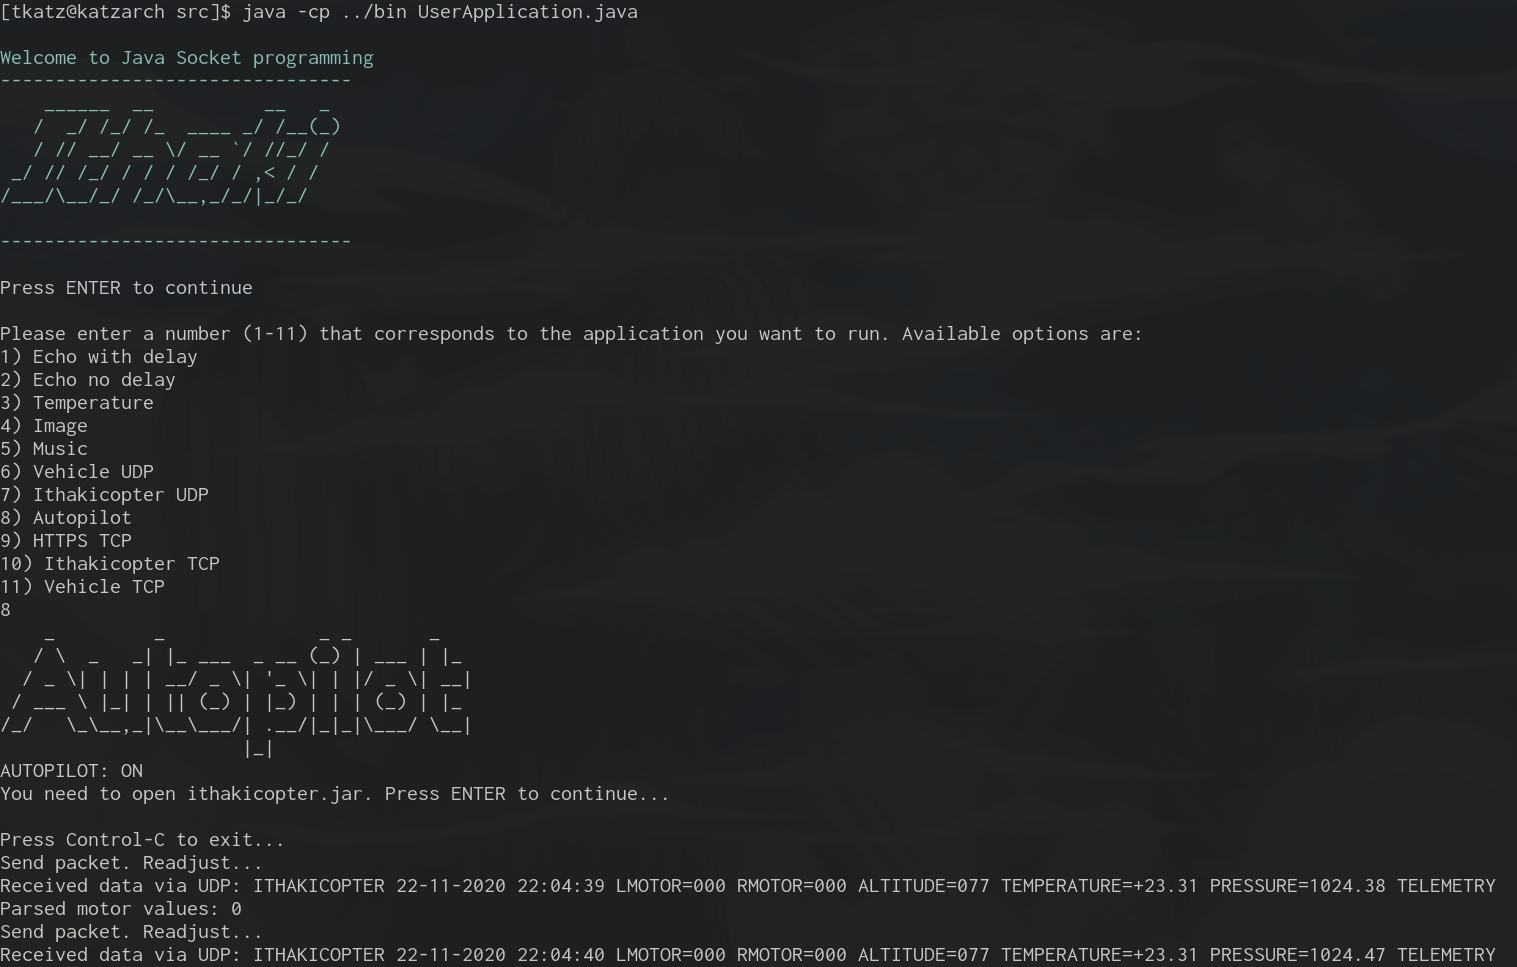
\includegraphics[width=\textwidth]{assets/ui.png}
	\caption{Εκτέλεση προγράμματος σε κέλυφος Bash} 
    \label{fig:ui}
\end{figure}

\section{TCP and UDP}


\section{Statement of originality aka bibliography}
 
\end{document}
